%%%%%%%%%%%%%%%%%%%%%%%%%%%%%%%%%%%%%%%%%%%%%%%%%%%%%%%%%%%%%%%%%%%%%%%%%%%%%%%%
%2345678901234567890123456789012345678901234567890123456789012345678901234567890
%        1         2         3         4         5         6         7         8

%\documentclass[letterpaper, 10 pt, conference]{ieeeconf}  % Comment this line out
                                                          % if you need a4paper
%
\documentclass[a4paper, 10pt, conference]{ieeeconf}      % Use this line for a4
                                                          % paper

\IEEEoverridecommandlockouts                              % This command is only
                                                          % needed if you want to
                                                          % use the \thanks command
\overrideIEEEmargins
% See the \addtolength command later in the file to balance the column lengths
% on the last page of the document



% The following packages can be found on http:\\www.ctan.org
\usepackage{graphics} % for pdf, bitmapped graphics files
%\usepackage{epsfig} % for postscript graphics files
%\usepackage{mathptmx} % assumes new font selection scheme installed
%\usepackage{times} % assumes new font selection scheme installed
%\usepackage{amsmath} % assumes amsmath package installed
%\usepackage{amssymb}  % assumes amsmath package installed
\newcommand{\horrule}[1]{\rule{\linewidth}{#1}} 	% Horizontal rule

%mypackages
\usepackage{amsmath}
 \usepackage[table,xcdraw]{xcolor}
\usepackage[pdftex]{graphicx}
\usepackage[english]{babel}
\usepackage{geometry} 
\usepackage[utf8]{inputenc}
\usepackage{graphicx}
\usepackage{movie15}

\usepackage{fancyhdr} 
\usepackage{listings}
\definecolor{light-gray}{gray}{0.95}
\definecolor{pblue}{rgb}{0.13,0.13,1}
\definecolor{pgreen}{rgb}{0,0.5,0}
\definecolor{pred}{rgb}{0.9,0,0}
\definecolor{pgrey}{rgb}{0.46,0.45,0.48}
\lstset{language=Java,
		xleftmargin=0.5cm,
		framesep=4pt,
		framerule=0pt,
		stepnumber=1,
		numbersep=8pt,
		showstringspaces=false,
		breaklines=true,
		frameround=ftff,
		frame=single,
		belowcaptionskip=5em,
		belowskip=3em,
	showspaces=false,
	 backgroundcolor=\color{light-gray},
	showtabs=false,
	breaklines=true,
	showstringspaces=false,
	breakatwhitespace=true,
	commentstyle=\color{pgreen},
	keywordstyle=\color{pblue},
	stringstyle=\color{pred},
	basicstyle=\ttfamily
}

\usepackage{wrapfig}

\usepackage{multicol}
\usepackage[hyperfootnotes=false]{hyperref}
\hypersetup{
	colorlinks,
	citecolor=black,
	filecolor=black,
	linkcolor=black,
	colorlinks=false,
	urlbordercolor=white,
	citebordercolor=black,
	linkbordercolor = white
}
\title{
		%\vspace{-1in} 	
		\usefont{OT1}{bch}{b}{n}
		\normalfont \normalsize \textsc{University of Illinois At Chicago\\CS559 - Neural Networks - Fall 2015} \\ [25pt]
		\horrule{2pt} \\[0.4cm]
		\huge Project Report \\
		\horrule{2pt} \\[0.3cm]
}
\author{
		\normalfont 								\large
        M.S. student \textit{Umberto Di Fabrizio}\\		\normalsize
       % \today \\[0.5cm]
}
\date{}

\begin{document}

\maketitle
\thispagestyle{empty}
\pagestyle{empty}


%%%%%%%%%%%%%%%%%%%%%%%%%%%%%%%%%%%%%%%%%%%%%%%%%%%%%%%%%%%%%%%%%%%%%%%%%%%%%%%%
\begin{abstract}
The protein superfamily classification problem, which consists of determining the superfamily membership
of a given unknown protein sequence, is very important for a biologist. In this work, the classification task is tackled using several ANN (Backprop, CNN, LAMSTAR) which all reach above 95\% of accuracy and are compared with respect to their execution time. The goal
is to predict the family of novel protein sequences based on the sequence only. The results obtained are comparable to the state of the art and the methods can be further investigated to be adapted to a larger dataset of families.
\end{abstract}
%%%%%%%%%%%%%%%%%%%%%%%%%%%%%%%%%%%%%%%%%%%%%%%%%%%%%%%%%%%%%%%%%%%%%%%%%%%%%%%%
\section{INTRODUCTION}
Bioinformatics has been growing in the last three decades\cite{Efficient} given the huge amount of biological data that is continuously gathered, mainly about DNA, RNA and proteins. The volume of data generated from project such as The Human Genome Project\cite{human}(1990-2003) has strengthen the collaboration between the computer scientist community and the biologist one.\\
One of the most challenging problem is to classify protein accordingly to their function or by their family or superfamily. Protein sequences are composed by an unique sequence of 20 amino acids which determines the protein function. They carry out fundamental roles for the cells functions ( basically represent the blueprint of the cell), infact they determine the shape and the structure of the cell.\\ Each protein encode a certain function which depends on its structure and amino acids sequence but can only be completely understood with experiments. Those experiments are costly and slow thus they cannot keep pace with the amount of information available and which needs to be annotated.\\
The challenge that has been tackled is to classify proteins into functional or structural existing superfamilies so that the annotation process can be automated. \\  
A protein superfamily is a set of proteins for which common ancestry can be inferred so they possed sequence or structural homology. 
In a superfamily classification, an unlabeled protein sequence may belong
to any of the superfamily from a set of known superfamilies. This classification is enormously useful because similar protein sequences exhibit almost the same biological structure and function, more importantly one of the main reason is treating and preventing genetic disease as well as drug discovery, prediction of molecular function and medical diagnosis.

\section{BACKGROUND}
Several methods have been investigated in order to solve the superfamily classification problem: determining the superfamily membership of a given unknown protein sequence.
BLAST (Basic Local Alignment Search Tool) \cite{blast} is a
tool that uses direct modelling, performing a search of homologie
between sequences. This software explores the local
alignment in pairs to measure the similarity between sequences.
The classification is done based on the alignment
which had the greatest punctuation.

Another method that uses direct modelling is the HMM
Hidden Markov Models that is widely used for probabilistic
modelling of family of proteins. It uses probabilistic values
to score how much an unkown protein belongs to a given
family.

A Fuzzy ARTMAP model, a machine learning method has been proposed used to classify the protein sequence\cite{fuzzy}.

The use of Neural Networks to tackle this problem has been successfully presented in the work by C.H.Wu at al.\cite{wu1992}\cite{wu1995}\cite{wu1996} and an introductory survey of neural networks applied to genome problems can be found in the book by C.H.Wu and Jerry W. McLarty\cite{bookWu}. The book explains the basic idea of neural networks presenting the different kinds of network that can be used and gives meaningful example on how to use them.\\
The process of protein classification using ANN can be
divided in two parts: (i) pre-processing: protein sequence
encoding; (ii) processing the protein classification using the
ANN.\\ The first step is very challenging, the reason is that protein sequences have different lengths and can even be very long (\textasciitilde
1000) whilst the neural network has a fixed amount of inputs and can hardly handle missing inputs. The methods of encoding can be basically dived in two types\cite{bookWu}: direct or indirect. The direct encoding basically translate each amino acid into a binary vector\footnote{other techniques will be presented later} accordingly to the one-hot encoding, this means that given that we have 20 possible amino acids then each of them will be represented by a vector of 20 bits with only one position at '1' and all the rest with '0'. Of course this kind of encoding is not feasible in the common case because a protein sequence with 300 amino acid will be translated with 20*300=6000 binary inputs.\\
The indirect encoding tries to extract useful features from the protein sequence in order to give meaningful inputs to the neural networks, one example is usually the n-gram hashing method\cite{wu1992}. This ngram method computes residue frequencies, the basic idead is that if we have a sequence \textit{Seq}='ACACTGAC' then the possible bi-gram are 'AA', 'AC', 'AT', 'AG', 'CC', 'CA, 'CT', 'CG', 'TT', 'TA, 'TC', 'TG', 'GG', 'GA', 'GT', 'GC', and for each of them the occurrences are counted, usually the approach involves also the mapping of the original sequence to a smaller alphabet. A summary table on the encoding pros and cons is shown in Table I\\

\begin{table*}[t]
\centering
\label{enc}
\caption{Comparison between direct and indirect protein sequence encoding}
\begin{tabular}{|
		>{}c |c|c|}
	\hline
	& Pros             & Cons                                                                                                                                  \\ \hline
	Direct   & Keeps the sequence order                 & Encoding is too large                                                                                                                                         \\ \hline
	Indirect & Independent of length of the biosequence & \begin{tabular}[c]{@{}c@{}}It is hard to find meaningful feature,\\ this requires domain knowledge.\\ The order of the sequence is not mantained\end{tabular} \\ \hline
\end{tabular}



\end{table*}

\newpage

\section{OUTLINE}
The idea is to exploit the power of the Deep Learning Neural Network in order to classify the protein in its family.\\
In section ~\nameref{sec:collection} it is explained where the data was collected from and which tools have been used, in section ~\nameref{sec:encoding} the encoding method to transform the sequence to numbers for the ANN is discussed.
Sections  ~\nameref{sec:bp}, ~\nameref{sec:cnn}, ~\nameref{sec:lamstar} discuss the design and structure of the ANNs employed to solve the problem, together with the choices that were made to optimize the execution time and the accuracy of the nets. Finally section ~\nameref{sec:results} presents the results and in ~\nameref{sec:conclusion} the contribution of the work are summarized and compared to the state of the art techniques.
\section{DATA COLLECTION}\label{sec:collection}

	The objective is to obtain for each superfamily or family the list of all the proteins that belong to that family and their complete protein sequence, an example of data is shown in table ~\ref{family}.\\
	This step is particularly tricky because there is not a database of protein sequences and families, or better there are several but they all have to be queried manually through a web interface. For this reason the data is scraped from the web sites (\href{http://prosite.expasy.org/}{http://prosite.expasy.org/}, \href{http://www.uniprot.org/uniprot/}{http://www.uniprot.org/uniprot/}) with the use of the Kimono platform\cite{kimono} and Rscripts. Automatizing this step is particularly useful in case any new superfamily data has to be collected.\\
	With this process 4 families have been chosen: \textit{ADH\_SHORT},\textit{ ABC\_TRANSPORTER\_2}, \textit{G\_TR\_2}, \textit{GLOBIN}, and for each of them 600 protein sequences have been collected. The overall dataset is thus made by 2400 protein sequences and it is divided between training(90\%) and testing(10\%).
	

\begin{table*}[t]
	\centering
	\caption{Example of protein sequences and their family}
	\label{family}
	\begin{tabular}{|c|c|}
		\hline
		\rowcolor[HTML]{FFFFFF} 
		Family                                      & Sequence                                                                                                                                                                                                                                                                                                                                                                                                                                                                                                                                                                                                                                                                        \\ \hline
		\cellcolor[HTML]{FFFFFF}ABC\_TRANSPORTER\_2 & \begin{tabular}[c]{@{}c@{}}MAEAPAKKLTVSATEVAVEIVNMNKWYGDFHVLRDINLKVMRGERIVIAGPSGSGKSTMI\\ RCINRLEEHQKGKIVVDGTELTNDLKKIDEVRREVGMVFQHFNLFPHLTILENCTLAPIW\\ VRKMPKKQAEEVAMHFLKRVKIPEQANKYPGQLSGGQQQRVAIARSLCMNPKIMLFDEPT\\ SALDPEMIKEVLDTMVGLAEEGMTMLCVTHEMGFARQVANRVIFMDQGQIVEQNEPAAFF\\ DNPQHERTKLFLSQILH\end{tabular}                                                                                                                                                                                                                                                                                                                                                           \\ \hline
		\cellcolor[HTML]{FFFFFF}ABC\_TRANSPORTER\_2 & \begin{tabular}[c]{@{}c@{}}MDKTRQTELVRWLKQHSTSAKRWLRISMLLGVVSGLLIIAQAWFLAVILQALIMEHTPRE\\ QLLTPFILLLAVFVLRALLTVIRERVGFRCGQVVRQEVRNMVLNKLQALGPVWVKGKPAG\\ SWATIVLEQIEDMQEYYSRYLPQMYLAGIIPIMILIAIFPFNWAAALILFATAPLIPIFM\\ ALVGLGAADANRRNFVALGRLSGSFLDRLRGLDTLRLFFREKAEVQQIRESTEDFRSRTM\\ EVLRMAFLSSGVLEFFASISIAIVAVYFGFSYLGELNFGSYGLPVTMFAGFLALILSPEF\\ FQPLRDLGTYYHAKAQAVGAAESLVTLLESDGEQKTETGDKTPQDKPIQIEANKLEIYSH\\ DGQRLVGPLDFTIEPQQRIAVFGQSGAGKSSLLNLLLGFLPYKGSIKINGDELKELCPDK\\ WRALIGWVGQNPHLPEQTLIENICLGKPTASEAEIQQAIDDAYVSEFLPMLPDGLNTRLG\\ DYAARLSVGQAQRVAVARTLLKPSRILLLDEPAASLDAHSEKRVMHTLNQLAQQQTTIMV\\ THLLEETVNYDQIWVMANGQIIQRGHYAQLSQSEGPFARLLAHRSEEL\end{tabular} \\ \hline
		ADH\_SHORT                                  & \begin{tabular}[c]{@{}c@{}}MMDWNNKNVVYVGGFSGFGYQVCQMMMKKPMKHLIVCSRMENVEMLKKLQAINTSVKVMF\\ VQMNIADYASIVKGVKQVIGHVGHVDVLINGVGGLADKDVETTVAVNLTGLINTTLMFMP\\ YMDKTQSGHGGMVVSISSVYGLEPGPAFSVYSAAKHGGIGFTRSMADEHLYHKTGVAFMC\\ ICPAMTSTELMMNKRDMNWMKWVPHSEEMWKMVMDAKMQTPEECAVNMMTAMEQAKNGAI\\ YICSTSGMKEITPTVYMH\end{tabular}                                                                                                                                                                                                                                                                                                                                                          \\ \hline
		ADH\_SHORT                                  & \begin{tabular}[c]{@{}c@{}}MTNRLQGKVALVTGGASGVGLEVVKLLLGEGAKVAFSDINEAAGQQLAAELGERSMFVRH\\ DVSSEADWTLVMAAVQRRLGTLNVLVNNAGILLPGDMETGRLEDFSRLLKINTESVFIGC\\ QQGIAAMKETGGSIINMASVSSWLPIEQYAGYSASKAAVSALTRAAALSCRKQGYAIRVN\\ SIHPDGIYTPMMQASLPKGVSKEMVLHDPKLNRAGRAYMPERIAQLVLFLASDESSVMSG\\ SELHADNSILGMGL\end{tabular}                                                                                                                                                                                                                                                                                                                                                              \\ \hline
	\end{tabular}
	
\end{table*}
\begin{figure}[thpb]
	\centering
	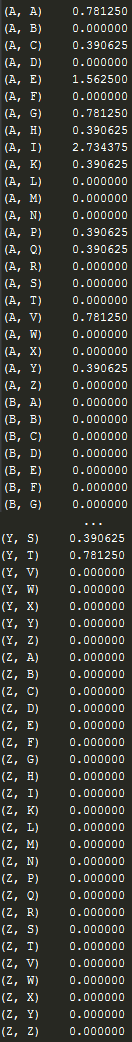
\includegraphics[scale=0.6]{1.png}
	\caption{Frequency bigrams for protein P00334.}
	\label{big}
\end{figure}
	
\section{DATA ENCODING}\label{sec:encoding}
	The sequences of proteins are encoded through the indirect method. The purpose is to extract as many information as possible from the protein without creating too many inputs for the neural network. The encoding adopted is a bigram hashing method as presented in \cite{bookWu} but the 20 amino acids are not mapped into 6 macro categories(as suggested), in order to keep as much information as possible. In this way we have 20x20 possible bigrams although there are also 3 special characters ('X','B','Z') that represent uncertainty of some amino acid base (e.g. X represent when it was not possible to detect the right amino acid), for this reason the total amount of inputs generated is 23x23=529. Notice that since we are using bigrams the number of inputs is the square of the number of possible amino acids, this is particular useful when we will reshape the input into a 23x23 matrix for the CNN.\\ A python script extracts the frequency of bigrams and normalize it on the length of the protein sequence, the information that we obtain represent a global feature of the sequence, an example of bigram frequency is shown in fig ~\ref{big}.



\clearpage
\newpage

\section{BACKPROPAGATION}\label{sec:bp}

	The backpropagation network as well as the other nets has been coded from scratch using Java.
	The input of the neural network is the encoded protein sequence, the output is the family of the protein.\\
	The network structure is shown in ~\ref{bp}: it is composed by an input layer of 6 neurons, an hidden layer of 5 neurons and an output layer of 4 neurons. The layer are fully connected so the total amount of weights to train are $529*6 + 6*5 + 5*4=3224$. The activation function in each layer is the tanh.\\ This particular configuration has been chosen for its simplicity, the network infact has been reduced to the minimum number of neurons required to have an high accuracy so that the execution time is minimized. In all the implementations that are presented (Backprop,CNN,LAMSTAR) the objective is to have an accuracy higher than 95\% minimizing the execution time that is notoriously the bottle neck of most ANN applications.\\
	The 4 output neurons represent the 4 chosen families using the one-hot encoding, and a result is considered correct only is each neuron has an absolute error less than 0.1.\\

\begin{figure}[thpb]
%	\centering
	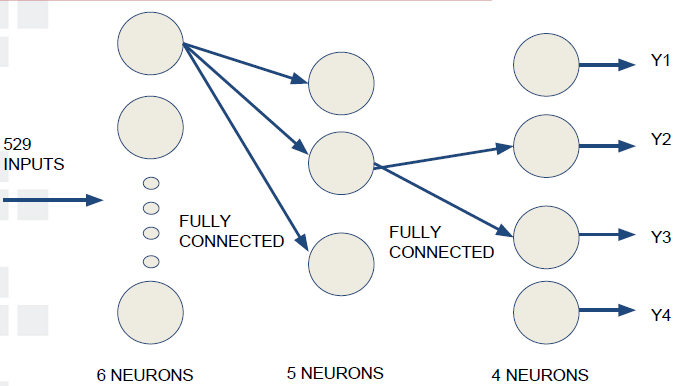
\includegraphics[scale=0.4]{bp.png}
	\caption{BackPropagation network structure.}
	\label{bp}
\end{figure}

\section{CONVOLUTIONAL NEURAL NETWORK}\label{sec:cnn}
The convolutional neural network is made by the following layers: a convolutional layer, a subsampling layer and a fully connected layer.The structure of the network is shown in fig  ~\ref{cnnNet}. 

\begin{figure}[thpb]
	\centering
	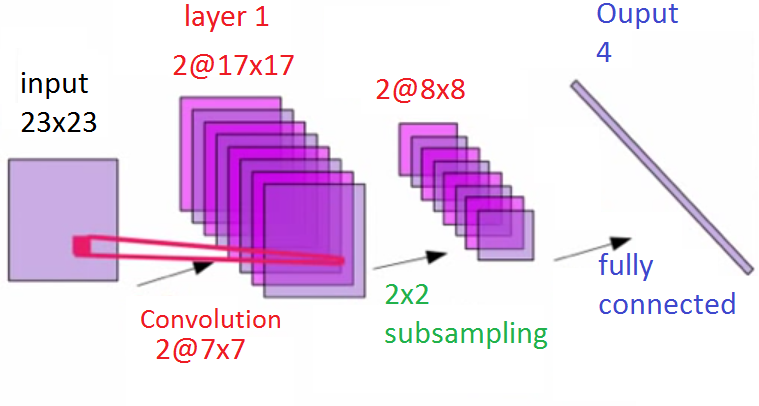
\includegraphics[scale=0.45]{cnn.png}
	\caption{Convolutional neural network structure.}
	\label{cnnNet}
\end{figure}
The input is a matrix 23x23 that represents the combinations of bigrams. The convolution is made with two 7x7 kernels (=filters) whose weights are learned through backpropagation, the result of the convolutional layer are two activation maps 17x17.
The subsampling layer is composed by two kernels 2x2 that apply a max pooling in order to produce two outputs 8x8. Finally the output is reshaped (note that this
is not a layer by itself but it is just a geometrical
transformation to connected the subsampling to
the fully connected layer) into a vector of 2x8x8 inputs and fully connected to the output layer which is composed by 4 output neurons. The activation function used in this net is the tanh.\\
\textbf{Convolution operation:}\\
The neurons of a convolutional layer are linked
to the previous ones through an operation of
convolution. In contrast with the neurons of a fully
connected layers, that can be disposed in vectors,
neurons of convolutional layers are disposed in
matrices. In order to compute the convolution,
a matrix kernel (the weights of the convolution)
is put over an area of neurons of the previous
layer and each input is multiplied with the corresponding
kernel weight (the filter) to generate the
output, this operations is shown in figure  ~\ref{conv}.\\
\textbf{Pooling operation:}\\ The pooling used is the
max-pooling which means that for each submatrix
(2x2) of the input layer the pooling layer extracts
only one value that is the maximum of the 4, in
this way the matrix dimension is reduced.\\
The network has been trained with a learning
rate = 0.01 which has been selected by exploring the range [0.01-0.05]. The weights and bias of the
network are initialized randomly by the framework
used : Torch\cite{torch} (based on Lua\cite{Lua}). The weights and biases are
then trained using the backpropagation algorithm
(extended for convolutoinal and subsampling layers)
and accordingly to the Minimum Squared
Error (MSE) error function.
Given the layer described in the previous section
we can count the total number of weights and
biases, we will se how the fact that the convolution
shares weights will lead to a small number of
weights to be trained compared to backpropagation:\\
weights:
\begin{itemize}
	\item 2 convolutional filters 7by7 = 98
	\item fully connected to 4 output neurons 64*2*4
	\item bias: 2 convolutional filters 7by7 = 2
	\item bias: fully connected to 4 output neurons = 4
\end{itemize}
The sum of weights to be trained is thus 616
which is much lower than the 3224 weights needed
in the backpropagation network.

\begin{figure}[thpb]
	\centering
	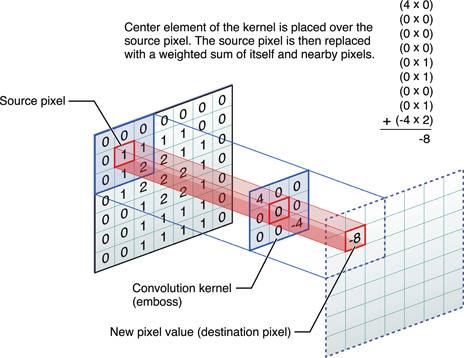
\includegraphics[scale=0.45]{conv.jpg}
	\caption{Convolution operation example.}
	\label{conv}
\end{figure}
\section{LAMSTAR}\label{sec:lamstar}
The LAMSTAR network can be implemented both in its classical version or with the normalization feature. In this work the version1 was performing very poorly (65\%) compared to the backpropagation and the convolutional one, so the normalized version has been configured and analyzed.\\
The chosen network architecture has been exploited with two configurations, in the first case the input matrix 23x23 has been divided into 23 subwords representing the rows plus 23 subwords representing the columns for a total of 46 input subwords, in the second case only the rows have been used as subwords. By testing the two types of architectures I noticed that the performances were the same but the LAMSTAR with only the rows as subwords was faster so it has been selected for further tests which are shown in the RESULTS section.\\
The network has 23 SOM modules.
The number of neurons implemented in each
SOM module is dynamic, according to the typical
LAMSTAR design. A neuron is added to each
SOM module only if it necessary to recognize a
new pattern, the discussion about the threshold used is in the next section.
No links between SOM modules have been implemented because not necessary in this case. Also the forgetting feature of LAMSTAR
has been avoided, since was not relevant
to the kind the problem addressed.
Indeed, one of the the configurations of the network is the \textit{reward} factor and the \textit{punishment} factor.\\
The network output is composed by 4 neurons, so anytime a neuron is chosen as winner its weights are rewarded 20 times the \textit{reward} factor which has been fixed to 0.05; the \textit{punishment} factor has been fixed to -0.025 because this lead to a higher performance of the network since during the test it emerged that some weights were punished too strongly.
The basic network structure is shown in figure ~\ref{lamstar}.
\begin{figure}[thpb]
	\centering
	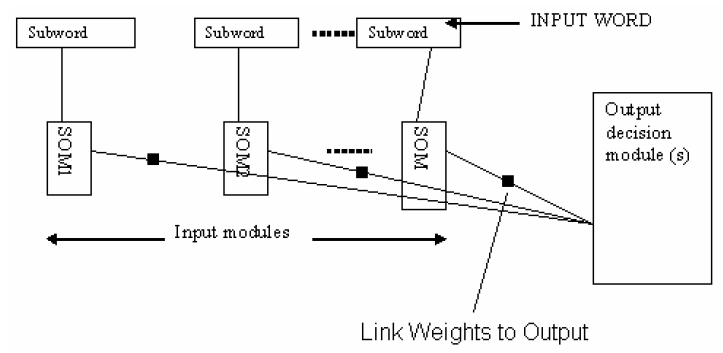
\includegraphics[scale=0.45]{lamstar.png}
	\caption{LAMSTAR network structure.}
	\label{lamstar}
\end{figure}
\section{RESULTS}\label{sec:results}
The purpose of this work is to minimize the execution time of the network keeping an high accuracy, for this reason all of the nets have been trained to reach an accuracy higher than 95\%. For each network several tests has been done regarding the amount of training data needed to reach 95\% of accuracy and the value of parameters such as : learning rate, number of kernels and epochs.\\
The backpropagation has been trained for 5 epochs and the result are shown in fig ~\ref{bpPlot}, the graph shows than the more training is used the quicker the network learns. The network execution times varies with the learning rate that has been tested between 0.1 and 1.5, the best results are obtain by a learning rate equal to 1 and the quickest training is reached with 70\% of the available training set. The final result for the backpropagation is an accuracy of 95\% in 98ms.\\
\begin{figure}[thpb]
	
	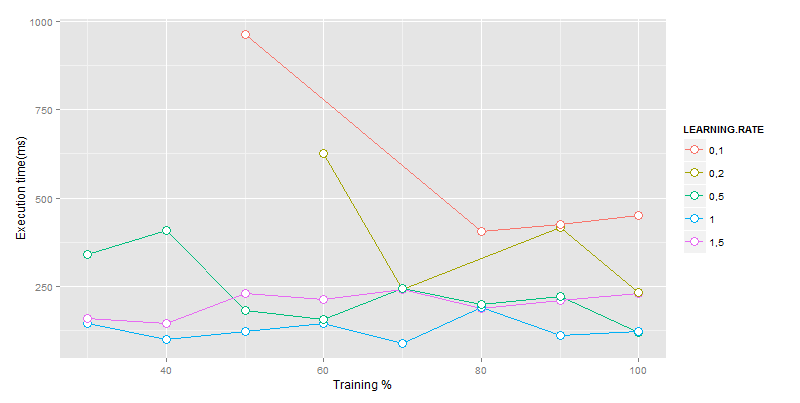
\includegraphics[scale=0.3]{plotBP.png}
	\caption{Execution time of backpropagation network for 95\% of accuracy for 5 epochs.}
	\label{bpPlot}
\end{figure}
As regard the CNN the parameter space has been meticulously tested to select the best values and the best result is achieved with 1 epoch training, learning rate 0.01, 2 convolutional kernels and using only 70\% of the training, the execution time in this case is 669ms.\\ Because both the CNN and the backpropagation have the highest results with 70\% of the training the conclusion is that with more training data the networks start to overfit so they fail to generalize and obtain a lower accuracy.\\
Finally the RESULT for LAMSTAR are shown in fig ~\ref{lamstarPlot}, the most important parameter for LAMSTAR has been the threshold error in the SOM layers, which means the highest distance between two vector in order to be associated to the same winning neuron. This is very important because it determines the degree of generalization of the SOM layer, moreover a higher threshold diminishes the execution time because there are less neurons in the SOM layers.
In the plot we see that the best performances are reached with a threshold error of 0.3 (a higher threshold decreases the accuracy of the network). In the end the lowest execution time of 372ms is obtained using 60\% of the training for 1 epoch.
\begin{figure}[thpb]
	
	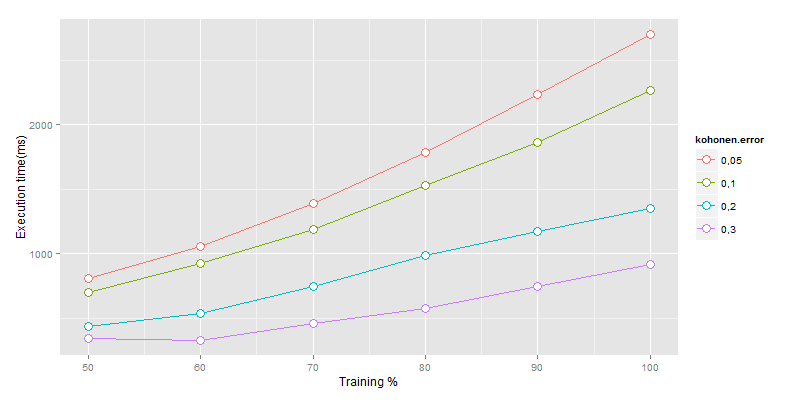
\includegraphics[scale=0.3]{plotLamstar2.png}
	\caption{Execution time of LAMSTAR network for 95\% of accuracy for 1 epoch.}
	\label{lamstarPlot}
\end{figure}

The table ~\ref{comp} presents a final comparison between the three networks. The Backpropagation is the quickest to reach 95\% of accuracy although the number of weights to train is higher. The LAMSTAR network performs much better than the CNN using even less training data, which means that it can absorb more knowledge for each datapoint.
\begin{table}[]
	\centering
	\caption{Comparison between the ANNs with accuracy 95\%}
	\label{comp}
	\begin{tabular}{|c|c|c|c|}
		\hline
		ANN                 & Backpropagation & CNN & LAMSTAR \\ \hline
		Execution Time (ms) & 98              & 669 & 372     \\ \hline
	\end{tabular}
\end{table}
\section{CONCLUSION}\label{sec:conclusion}
In this work it has been tackled the problem of protein superfamily classification which consist on determining the family of a given protein. The analysis compares three types of ANN which all perform above 95\% of accuracy and shows that the quickest network is the backpropagation with an execution time of 98ms while the LAMSTAR is faster than the CNN by 180\%.\\
As far as my knowledge goes this work is comparable to the state of the art solution\cite{probab} which report a precision of 97.6\% for the same problem using a Probabilistic Neural Network. Anyway it is harder to compare this result with the work of Wu et al.\cite{wu1992} that uses an ensemble of Neural Netoworks for the same classification problem on a dataset of 620 superfamilies obtaining an accuracy of 90\%.
\section{CODE}
The code:
\begin{itemize}
	\item  R scripts and python scripts for the data collection and preprocessing
	\item Java for the backpropagation and LAMSTAR
	\item Torch for the CNN
\end{itemize}
is available at: \href{https://github.com/umbertoDifa/protein-family-classification-ann}{https://github.com/umbertoDifa/protein-family-classification-ann}


\clearpage
\newpage
\begin{thebibliography}{99}

\bibitem{graupe}D.Graupe, Principles of Artificial Neural Networks, 3nd ed., Advanced Series in Circuits and System-Vol.7

\bibitem{Efficient}Efficient Feature Selection and Classification of Protein Sequence Data in Bioinformatics,Muhammad Javed Iqbal et al., 2014

\bibitem{human}\href{https://www.genome.gov/12011238}{https://www.genome.gov/12011238}

\bibitem{blast}Basic local alignment tool,S. Altschul et al., 1990
\bibitem{wu1992}Protein classification artificial neural system, C. H. Wu et al, 1992
\bibitem{wu1995}Neural Networks for Full-Scale Protein Sequence, C. H. Wu et al, 1995
\bibitem{wu1996}Motif identification neural design for rapid and sensitive protein family search, C. H. Wu et al,1996
\bibitem{fuzzy}Multi-class Protein Sequence Classification Using Fuzzy ARTMAP,Shakir Mohamed et al.,2006

\bibitem{bookWu}Neural Networks and Genome Informatics
\bibitem{kimono}\href{https://www.kimonolabs.com/}{https://www.kimonolabs.com/}
\bibitem{torch}Torch Framework at: http://torch.ch/
\bibitem{Lua}Lua Language at :www.lua.org
\bibitem{probab}A Probabilistic Neural Network approach for
Protein Superfamily Classification, Pv Nageswara Rao et al., 2009

\end{thebibliography}

\end{document}
